\documentclass[twoside]{book}

% Packages required by doxygen
\usepackage{fixltx2e}
\usepackage{calc}
\usepackage{doxygen}
\usepackage[export]{adjustbox} % also loads graphicx
\usepackage{graphicx}
\usepackage[utf8]{inputenc}
\usepackage{makeidx}
\usepackage{multicol}
\usepackage{multirow}
\PassOptionsToPackage{warn}{textcomp}
\usepackage{textcomp}
\usepackage[nointegrals]{wasysym}
\usepackage[table]{xcolor}

% Font selection
\usepackage[T1]{fontenc}
\usepackage[scaled=.90]{helvet}
\usepackage{courier}
\usepackage{amssymb}
\usepackage{sectsty}
\renewcommand{\familydefault}{\sfdefault}
\allsectionsfont{%
  \fontseries{bc}\selectfont%
  \color{darkgray}%
}
\renewcommand{\DoxyLabelFont}{%
  \fontseries{bc}\selectfont%
  \color{darkgray}%
}
\newcommand{\+}{\discretionary{\mbox{\scriptsize$\hookleftarrow$}}{}{}}

% Page & text layout
\usepackage{geometry}
\geometry{%
  a4paper,%
  top=2.5cm,%
  bottom=2.5cm,%
  left=2.5cm,%
  right=2.5cm%
}
\tolerance=750
\hfuzz=15pt
\hbadness=750
\setlength{\emergencystretch}{15pt}
\setlength{\parindent}{0cm}
\setlength{\parskip}{3ex plus 2ex minus 2ex}
\makeatletter
\renewcommand{\paragraph}{%
  \@startsection{paragraph}{4}{0ex}{-1.0ex}{1.0ex}{%
    \normalfont\normalsize\bfseries\SS@parafont%
  }%
}
\renewcommand{\subparagraph}{%
  \@startsection{subparagraph}{5}{0ex}{-1.0ex}{1.0ex}{%
    \normalfont\normalsize\bfseries\SS@subparafont%
  }%
}
\makeatother

% Headers & footers
\usepackage{fancyhdr}
\pagestyle{fancyplain}
\fancyhead[LE]{\fancyplain{}{\bfseries\thepage}}
\fancyhead[CE]{\fancyplain{}{}}
\fancyhead[RE]{\fancyplain{}{\bfseries\leftmark}}
\fancyhead[LO]{\fancyplain{}{\bfseries\rightmark}}
\fancyhead[CO]{\fancyplain{}{}}
\fancyhead[RO]{\fancyplain{}{\bfseries\thepage}}
\fancyfoot[LE]{\fancyplain{}{}}
\fancyfoot[CE]{\fancyplain{}{}}
\fancyfoot[RE]{\fancyplain{}{\bfseries\scriptsize Generated by Doxygen }}
\fancyfoot[LO]{\fancyplain{}{\bfseries\scriptsize Generated by Doxygen }}
\fancyfoot[CO]{\fancyplain{}{}}
\fancyfoot[RO]{\fancyplain{}{}}
\renewcommand{\footrulewidth}{0.4pt}
\renewcommand{\chaptermark}[1]{%
  \markboth{#1}{}%
}
\renewcommand{\sectionmark}[1]{%
  \markright{\thesection\ #1}%
}

% Indices & bibliography
\usepackage{natbib}
\usepackage[titles]{tocloft}
\setcounter{tocdepth}{3}
\setcounter{secnumdepth}{5}
\makeindex

% Hyperlinks (required, but should be loaded last)
\usepackage{ifpdf}
\ifpdf
  \usepackage[pdftex,pagebackref=true]{hyperref}
\else
  \usepackage[ps2pdf,pagebackref=true]{hyperref}
\fi
\hypersetup{%
  colorlinks=true,%
  linkcolor=blue,%
  citecolor=blue,%
  unicode%
}

% Custom commands
\newcommand{\clearemptydoublepage}{%
  \newpage{\pagestyle{empty}\cleardoublepage}%
}

\usepackage{caption}
\captionsetup{labelsep=space,justification=centering,font={bf},singlelinecheck=off,skip=4pt,position=top}

%===== C O N T E N T S =====

\begin{document}

% Titlepage & ToC
\hypersetup{pageanchor=false,
             bookmarksnumbered=true,
             pdfencoding=unicode
            }
\pagenumbering{roman}
\begin{titlepage}
\vspace*{7cm}
\begin{center}%
{\Large My Project }\\
\vspace*{1cm}
{\large Generated by Doxygen 1.8.11}\\
\end{center}
\end{titlepage}
\clearemptydoublepage
\tableofcontents
\clearemptydoublepage
\pagenumbering{arabic}
\hypersetup{pageanchor=true}

%--- Begin generated contents ---
\chapter{Class Index}
\section{Class List}
Here are the classes, structs, unions and interfaces with brief descriptions\+:\begin{DoxyCompactList}
\item\contentsline{section}{\hyperlink{structnode}{node} }{\pageref{structnode}}{}
\item\contentsline{section}{\hyperlink{structnode1}{node1} }{\pageref{structnode1}}{}
\item\contentsline{section}{\hyperlink{structnode__info}{node\+\_\+info} }{\pageref{structnode__info}}{}
\end{DoxyCompactList}

\chapter{File Index}
\section{File List}
Here is a list of all files with brief descriptions\+:\begin{DoxyCompactList}
\item\contentsline{section}{\hyperlink{Lab1_8c}{Lab1.\+c} }{\pageref{Lab1_8c}}{}
\end{DoxyCompactList}

\chapter{Class Documentation}
\hypertarget{classHashEntry}{}\section{Hash\+Entry Class Reference}
\label{classHashEntry}\index{Hash\+Entry@{Hash\+Entry}}
\subsection*{Public Member Functions}
\begin{DoxyCompactItemize}
\item 
\hyperlink{classHashEntry_ac78ceaa6e531ebbf3cef97fe9f649222}{Hash\+Entry} (int \hyperlink{classHashEntry_ae861ef0082b8111cb9e581d3961ab9b2}{key}, int \hyperlink{classHashEntry_aa225f361520a57dbaf93e9d00bf69490}{value})
\end{DoxyCompactItemize}
\subsection*{Public Attributes}
\begin{DoxyCompactItemize}
\item 
int \hyperlink{classHashEntry_ae861ef0082b8111cb9e581d3961ab9b2}{key}
\item 
int \hyperlink{classHashEntry_aa225f361520a57dbaf93e9d00bf69490}{value}
\end{DoxyCompactItemize}


\subsection{Constructor \& Destructor Documentation}
\index{Hash\+Entry@{Hash\+Entry}!Hash\+Entry@{Hash\+Entry}}
\index{Hash\+Entry@{Hash\+Entry}!Hash\+Entry@{Hash\+Entry}}
\subsubsection[{\texorpdfstring{Hash\+Entry(int key, int value)}{HashEntry(int key, int value)}}]{\setlength{\rightskip}{0pt plus 5cm}Hash\+Entry\+::\+Hash\+Entry (
\begin{DoxyParamCaption}
\item[{int}]{key, }
\item[{int}]{value}
\end{DoxyParamCaption}
)\hspace{0.3cm}{\ttfamily [inline]}}\hypertarget{classHashEntry_ac78ceaa6e531ebbf3cef97fe9f649222}{}\label{classHashEntry_ac78ceaa6e531ebbf3cef97fe9f649222}

\begin{DoxyCode}
20         \{
21             this->\hyperlink{classHashEntry_ae861ef0082b8111cb9e581d3961ab9b2}{key} = \hyperlink{classHashEntry_ae861ef0082b8111cb9e581d3961ab9b2}{key};
22             this->\hyperlink{classHashEntry_aa225f361520a57dbaf93e9d00bf69490}{value} = \hyperlink{classHashEntry_aa225f361520a57dbaf93e9d00bf69490}{value};
23         \}
\end{DoxyCode}


\subsection{Member Data Documentation}
\index{Hash\+Entry@{Hash\+Entry}!key@{key}}
\index{key@{key}!Hash\+Entry@{Hash\+Entry}}
\subsubsection[{\texorpdfstring{key}{key}}]{\setlength{\rightskip}{0pt plus 5cm}int Hash\+Entry\+::key}\hypertarget{classHashEntry_ae861ef0082b8111cb9e581d3961ab9b2}{}\label{classHashEntry_ae861ef0082b8111cb9e581d3961ab9b2}
\index{Hash\+Entry@{Hash\+Entry}!value@{value}}
\index{value@{value}!Hash\+Entry@{Hash\+Entry}}
\subsubsection[{\texorpdfstring{value}{value}}]{\setlength{\rightskip}{0pt plus 5cm}int Hash\+Entry\+::value}\hypertarget{classHashEntry_aa225f361520a57dbaf93e9d00bf69490}{}\label{classHashEntry_aa225f361520a57dbaf93e9d00bf69490}


The documentation for this class was generated from the following file\+:\begin{DoxyCompactItemize}
\item 
\hyperlink{HashTable_8cpp}{Hash\+Table.\+cpp}\end{DoxyCompactItemize}

\hypertarget{classHashMap}{}\section{Hash\+Map Class Reference}
\label{classHashMap}\index{Hash\+Map@{Hash\+Map}}


Collaboration diagram for Hash\+Map\+:
\nopagebreak
\begin{figure}[H]
\begin{center}
\leavevmode
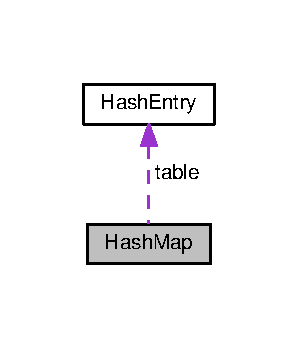
\includegraphics[width=143pt]{classHashMap__coll__graph}
\end{center}
\end{figure}
\subsection*{Public Member Functions}
\begin{DoxyCompactItemize}
\item 
\hyperlink{classHashMap_a3ae91705aa3ebfff22ce92e3c7797050}{Hash\+Map} ()
\item 
int \hyperlink{classHashMap_af676e8e12150e2f94ed7766103795f84}{Hash\+Func} (int key)
\item 
void \hyperlink{classHashMap_aa595b4e98a9ec68efa0ee9fe75126186}{Insert} (int key, int value)
\item 
int \hyperlink{classHashMap_a2801980039df1862de284ce00cb6d1f3}{Search} (int key)
\item 
void \hyperlink{classHashMap_a021573afbb91afef3b30e90d22aed366}{Remove} (int key)
\item 
\hyperlink{classHashMap_a7120321a936e8018fd276bcd4b4da3b8}{$\sim$\+Hash\+Map} ()
\end{DoxyCompactItemize}
\subsection*{Private Attributes}
\begin{DoxyCompactItemize}
\item 
\hyperlink{classHashEntry}{Hash\+Entry} $\ast$$\ast$ \hyperlink{classHashMap_a17f8fbff625a697ac94039b4a1c6cce4}{table}
\end{DoxyCompactItemize}


\subsection{Constructor \& Destructor Documentation}
\index{Hash\+Map@{Hash\+Map}!Hash\+Map@{Hash\+Map}}
\index{Hash\+Map@{Hash\+Map}!Hash\+Map@{Hash\+Map}}
\subsubsection[{\texorpdfstring{Hash\+Map()}{HashMap()}}]{\setlength{\rightskip}{0pt plus 5cm}Hash\+Map\+::\+Hash\+Map (
\begin{DoxyParamCaption}
{}
\end{DoxyParamCaption}
)\hspace{0.3cm}{\ttfamily [inline]}}\hypertarget{classHashMap_a3ae91705aa3ebfff22ce92e3c7797050}{}\label{classHashMap_a3ae91705aa3ebfff22ce92e3c7797050}

\begin{DoxyCode}
35     \{
36             \hyperlink{classHashMap_a17f8fbff625a697ac94039b4a1c6cce4}{table} = \textcolor{keyword}{new} \hyperlink{classHashEntry}{HashEntry} * [\hyperlink{HashTable_8cpp_ada4ebb227211f96616c9e6681a944bc1}{TABLE\_SIZE}];
37             \textcolor{keywordflow}{for} (\textcolor{keywordtype}{int} i = 0; i< \hyperlink{HashTable_8cpp_ada4ebb227211f96616c9e6681a944bc1}{TABLE\_SIZE}; i++)
38             \{
39                 \hyperlink{classHashMap_a17f8fbff625a697ac94039b4a1c6cce4}{table}[i] = NULL;
40             \}
41         \}
\end{DoxyCode}
\index{Hash\+Map@{Hash\+Map}!````~Hash\+Map@{$\sim$\+Hash\+Map}}
\index{````~Hash\+Map@{$\sim$\+Hash\+Map}!Hash\+Map@{Hash\+Map}}
\subsubsection[{\texorpdfstring{$\sim$\+Hash\+Map()}{~HashMap()}}]{\setlength{\rightskip}{0pt plus 5cm}Hash\+Map\+::$\sim$\+Hash\+Map (
\begin{DoxyParamCaption}
{}
\end{DoxyParamCaption}
)\hspace{0.3cm}{\ttfamily [inline]}}\hypertarget{classHashMap_a7120321a936e8018fd276bcd4b4da3b8}{}\label{classHashMap_a7120321a936e8018fd276bcd4b4da3b8}

\begin{DoxyCode}
103     \{
104             \textcolor{keywordflow}{for} (\textcolor{keywordtype}{int} i = 0; i < \hyperlink{HashTable_8cpp_ada4ebb227211f96616c9e6681a944bc1}{TABLE\_SIZE}; i++)
105             \{
106                 \textcolor{keywordflow}{if} (\hyperlink{classHashMap_a17f8fbff625a697ac94039b4a1c6cce4}{table}[i] != NULL)
107                     \textcolor{keyword}{delete} \hyperlink{classHashMap_a17f8fbff625a697ac94039b4a1c6cce4}{table}[i];
108                 \textcolor{keyword}{delete}[] \hyperlink{classHashMap_a17f8fbff625a697ac94039b4a1c6cce4}{table};
109             \}
110         \}
\end{DoxyCode}


\subsection{Member Function Documentation}
\index{Hash\+Map@{Hash\+Map}!Hash\+Func@{Hash\+Func}}
\index{Hash\+Func@{Hash\+Func}!Hash\+Map@{Hash\+Map}}
\subsubsection[{\texorpdfstring{Hash\+Func(int key)}{HashFunc(int key)}}]{\setlength{\rightskip}{0pt plus 5cm}int Hash\+Map\+::\+Hash\+Func (
\begin{DoxyParamCaption}
\item[{int}]{key}
\end{DoxyParamCaption}
)\hspace{0.3cm}{\ttfamily [inline]}}\hypertarget{classHashMap_af676e8e12150e2f94ed7766103795f84}{}\label{classHashMap_af676e8e12150e2f94ed7766103795f84}

\begin{DoxyCode}
46         \{
47             \textcolor{keywordflow}{return} key % \hyperlink{HashTable_8cpp_ada4ebb227211f96616c9e6681a944bc1}{TABLE\_SIZE};
48         \}
\end{DoxyCode}
\index{Hash\+Map@{Hash\+Map}!Insert@{Insert}}
\index{Insert@{Insert}!Hash\+Map@{Hash\+Map}}
\subsubsection[{\texorpdfstring{Insert(int key, int value)}{Insert(int key, int value)}}]{\setlength{\rightskip}{0pt plus 5cm}void Hash\+Map\+::\+Insert (
\begin{DoxyParamCaption}
\item[{int}]{key, }
\item[{int}]{value}
\end{DoxyParamCaption}
)\hspace{0.3cm}{\ttfamily [inline]}}\hypertarget{classHashMap_aa595b4e98a9ec68efa0ee9fe75126186}{}\label{classHashMap_aa595b4e98a9ec68efa0ee9fe75126186}

\begin{DoxyCode}
53     \{
54             \textcolor{keywordtype}{int} hash = \hyperlink{classHashMap_af676e8e12150e2f94ed7766103795f84}{HashFunc}(key);
55             \textcolor{keywordflow}{while} (\hyperlink{classHashMap_a17f8fbff625a697ac94039b4a1c6cce4}{table}[hash] != NULL && \hyperlink{classHashMap_a17f8fbff625a697ac94039b4a1c6cce4}{table}[hash]->key != key)
56             \{
57                 hash = \hyperlink{classHashMap_af676e8e12150e2f94ed7766103795f84}{HashFunc}(hash + 1);
58             \}
59             \textcolor{keywordflow}{if} (\hyperlink{classHashMap_a17f8fbff625a697ac94039b4a1c6cce4}{table}[hash] != NULL)
60                 \textcolor{keyword}{delete} \hyperlink{classHashMap_a17f8fbff625a697ac94039b4a1c6cce4}{table}[hash];
61             \hyperlink{classHashMap_a17f8fbff625a697ac94039b4a1c6cce4}{table}[hash] = \textcolor{keyword}{new} \hyperlink{classHashEntry}{HashEntry}(key, value);
62     \}
\end{DoxyCode}
\index{Hash\+Map@{Hash\+Map}!Remove@{Remove}}
\index{Remove@{Remove}!Hash\+Map@{Hash\+Map}}
\subsubsection[{\texorpdfstring{Remove(int key)}{Remove(int key)}}]{\setlength{\rightskip}{0pt plus 5cm}void Hash\+Map\+::\+Remove (
\begin{DoxyParamCaption}
\item[{int}]{key}
\end{DoxyParamCaption}
)\hspace{0.3cm}{\ttfamily [inline]}}\hypertarget{classHashMap_a021573afbb91afef3b30e90d22aed366}{}\label{classHashMap_a021573afbb91afef3b30e90d22aed366}

\begin{DoxyCode}
83     \{
84         \textcolor{keywordtype}{int} hash = \hyperlink{classHashMap_af676e8e12150e2f94ed7766103795f84}{HashFunc}(key);
85         \textcolor{keywordflow}{while} (\hyperlink{classHashMap_a17f8fbff625a697ac94039b4a1c6cce4}{table}[hash] != NULL)
86         \{
87             \textcolor{keywordflow}{if} (\hyperlink{classHashMap_a17f8fbff625a697ac94039b4a1c6cce4}{table}[hash]->key == key)
88                 \textcolor{keywordflow}{break};
89             hash = \hyperlink{classHashMap_af676e8e12150e2f94ed7766103795f84}{HashFunc}(hash + 1);
90         \}
91             \textcolor{keywordflow}{if} (\hyperlink{classHashMap_a17f8fbff625a697ac94039b4a1c6cce4}{table}[hash] == NULL)
92         \{
93                 cout<<\textcolor{stringliteral}{"No Element found at key "}<<key<<endl;
94                 \textcolor{keywordflow}{return};
95             \}
96             \textcolor{keywordflow}{else}
97             \{
98                 \textcolor{keyword}{delete} \hyperlink{classHashMap_a17f8fbff625a697ac94039b4a1c6cce4}{table}[hash];
99             \}
100             cout<<\textcolor{stringliteral}{"Element Deleted"}<<endl;
101         \}
\end{DoxyCode}
\index{Hash\+Map@{Hash\+Map}!Search@{Search}}
\index{Search@{Search}!Hash\+Map@{Hash\+Map}}
\subsubsection[{\texorpdfstring{Search(int key)}{Search(int key)}}]{\setlength{\rightskip}{0pt plus 5cm}int Hash\+Map\+::\+Search (
\begin{DoxyParamCaption}
\item[{int}]{key}
\end{DoxyParamCaption}
)\hspace{0.3cm}{\ttfamily [inline]}}\hypertarget{classHashMap_a2801980039df1862de284ce00cb6d1f3}{}\label{classHashMap_a2801980039df1862de284ce00cb6d1f3}

\begin{DoxyCode}
67     \{
68         \textcolor{keywordtype}{int}  hash = \hyperlink{classHashMap_af676e8e12150e2f94ed7766103795f84}{HashFunc}(key);
69         \textcolor{keywordflow}{while} (\hyperlink{classHashMap_a17f8fbff625a697ac94039b4a1c6cce4}{table}[hash] != NULL && \hyperlink{classHashMap_a17f8fbff625a697ac94039b4a1c6cce4}{table}[hash]->key != key)
70         \{
71             hash = \hyperlink{classHashMap_af676e8e12150e2f94ed7766103795f84}{HashFunc}(hash + 1);
72         \}
73         \textcolor{keywordflow}{if} (\hyperlink{classHashMap_a17f8fbff625a697ac94039b4a1c6cce4}{table}[hash] == NULL)
74             \textcolor{keywordflow}{return} -1;
75         \textcolor{keywordflow}{else}
76             \textcolor{keywordflow}{return} \hyperlink{classHashMap_a17f8fbff625a697ac94039b4a1c6cce4}{table}[hash]->\hyperlink{classHashEntry_aa225f361520a57dbaf93e9d00bf69490}{value};
77         \}
\end{DoxyCode}


\subsection{Member Data Documentation}
\index{Hash\+Map@{Hash\+Map}!table@{table}}
\index{table@{table}!Hash\+Map@{Hash\+Map}}
\subsubsection[{\texorpdfstring{table}{table}}]{\setlength{\rightskip}{0pt plus 5cm}{\bf Hash\+Entry}$\ast$$\ast$ Hash\+Map\+::table\hspace{0.3cm}{\ttfamily [private]}}\hypertarget{classHashMap_a17f8fbff625a697ac94039b4a1c6cce4}{}\label{classHashMap_a17f8fbff625a697ac94039b4a1c6cce4}


The documentation for this class was generated from the following file\+:\begin{DoxyCompactItemize}
\item 
\hyperlink{HashTable_8cpp}{Hash\+Table.\+cpp}\end{DoxyCompactItemize}

\chapter{File Documentation}
\hypertarget{HashTable_8cpp}{}\section{Hash\+Table.\+cpp File Reference}
\label{HashTable_8cpp}\index{Hash\+Table.\+cpp@{Hash\+Table.\+cpp}}
{\ttfamily \#include $<$iostream$>$}\\*
{\ttfamily \#include $<$cstdlib$>$}\\*
{\ttfamily \#include $<$string$>$}\\*
{\ttfamily \#include $<$cstdio$>$}\\*
Include dependency graph for Hash\+Table.\+cpp\+:
\nopagebreak
\begin{figure}[H]
\begin{center}
\leavevmode
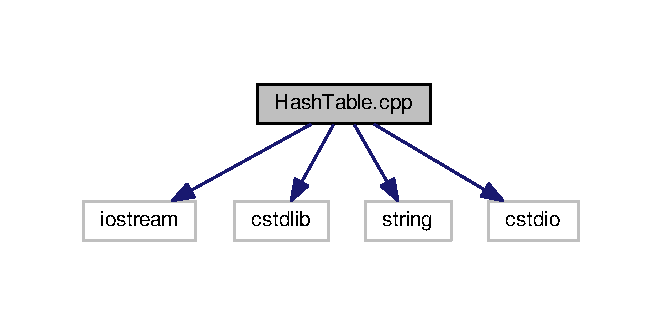
\includegraphics[width=318pt]{HashTable_8cpp__incl}
\end{center}
\end{figure}
\subsection*{Classes}
\begin{DoxyCompactItemize}
\item 
class \hyperlink{classHashEntry}{Hash\+Entry}
\item 
class \hyperlink{classHashMap}{Hash\+Map}
\end{DoxyCompactItemize}
\subsection*{Functions}
\begin{DoxyCompactItemize}
\item 
int \hyperlink{HashTable_8cpp_ae66f6b31b5ad750f1fe042a706a4e3d4}{main} ()
\end{DoxyCompactItemize}
\subsection*{Variables}
\begin{DoxyCompactItemize}
\item 
const int \hyperlink{HashTable_8cpp_ada4ebb227211f96616c9e6681a944bc1}{T\+A\+B\+L\+E\+\_\+\+S\+I\+ZE} = 128
\end{DoxyCompactItemize}


\subsection{Function Documentation}
\index{Hash\+Table.\+cpp@{Hash\+Table.\+cpp}!main@{main}}
\index{main@{main}!Hash\+Table.\+cpp@{Hash\+Table.\+cpp}}
\subsubsection[{\texorpdfstring{main()}{main()}}]{\setlength{\rightskip}{0pt plus 5cm}int main (
\begin{DoxyParamCaption}
{}
\end{DoxyParamCaption}
)}\hypertarget{HashTable_8cpp_ae66f6b31b5ad750f1fe042a706a4e3d4}{}\label{HashTable_8cpp_ae66f6b31b5ad750f1fe042a706a4e3d4}

\begin{DoxyCode}
116 \{
117     \hyperlink{classHashMap}{HashMap} hash;
118     \textcolor{keywordtype}{int} key, value;
119     \textcolor{keywordtype}{int} choice;
120     \textcolor{keywordflow}{while} (1)
121     \{
122         cout<<\textcolor{stringliteral}{"\(\backslash\)n----------------------"}<<endl;
123         cout<<\textcolor{stringliteral}{"Operations on Hash Table"}<<endl;
124         cout<<\textcolor{stringliteral}{"\(\backslash\)n----------------------"}<<endl;
125         cout<<\textcolor{stringliteral}{"1.Insert element into the table"}<<endl;
126         cout<<\textcolor{stringliteral}{"2.Search element from the key"}<<endl;
127         cout<<\textcolor{stringliteral}{"3.Delete element at a key"}<<endl;
128         cout<<\textcolor{stringliteral}{"4.Exit"}<<endl;
129         cout<<\textcolor{stringliteral}{"Enter your choice: "};
130         cin>>choice;
131         \textcolor{keywordflow}{switch}(choice)
132         \{
133         \textcolor{keywordflow}{case} 1:
134             cout<<\textcolor{stringliteral}{"Enter element to be inserted: "};
135             cin>>value;
136             cout<<\textcolor{stringliteral}{"Enter key at which element to be inserted: "};
137             cin>>key;
138             hash.\hyperlink{classHashMap_aa595b4e98a9ec68efa0ee9fe75126186}{Insert}(key, value);
139             \textcolor{keywordflow}{break};
140         \textcolor{keywordflow}{case} 2:
141             cout<<\textcolor{stringliteral}{"Enter key of the element to be searched: "};
142             cin>>key;
143             \textcolor{keywordflow}{if} (hash.\hyperlink{classHashMap_a2801980039df1862de284ce00cb6d1f3}{Search}(key) == -1)
144             \{
145             cout<<\textcolor{stringliteral}{"No element found at key "}<<key<<endl;
146             \textcolor{keywordflow}{continue};
147         \}
148         \textcolor{keywordflow}{else}
149         \{
150             cout<<\textcolor{stringliteral}{"Element at key "}<<key<<\textcolor{stringliteral}{" : "};
151             cout<<hash.\hyperlink{classHashMap_a2801980039df1862de284ce00cb6d1f3}{Search}(key)<<endl;
152         \}
153             \textcolor{keywordflow}{break};
154         \textcolor{keywordflow}{case} 3:
155             cout<<\textcolor{stringliteral}{"Enter key of the element to be deleted: "};
156             cin>>key;
157             hash.\hyperlink{classHashMap_a021573afbb91afef3b30e90d22aed366}{Remove}(key);
158             \textcolor{keywordflow}{break};
159         \textcolor{keywordflow}{case} 4:
160             exit(1);
161         \textcolor{keywordflow}{default}:
162            cout<<\textcolor{stringliteral}{"\(\backslash\)nEnter correct option\(\backslash\)n"};
163        \}
164     \}
165     \textcolor{keywordflow}{return} 0;
166 \}\end{DoxyCode}


Here is the call graph for this function\+:
\nopagebreak
\begin{figure}[H]
\begin{center}
\leavevmode
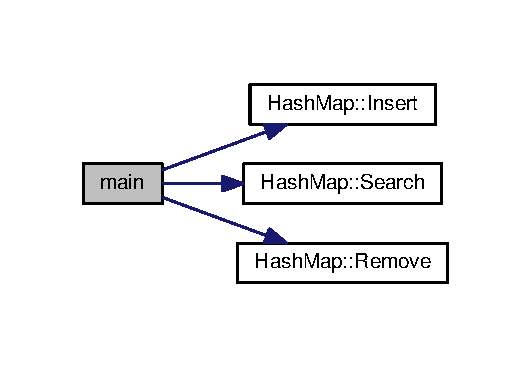
\includegraphics[width=255pt]{HashTable_8cpp_ae66f6b31b5ad750f1fe042a706a4e3d4_cgraph}
\end{center}
\end{figure}




\subsection{Variable Documentation}
\index{Hash\+Table.\+cpp@{Hash\+Table.\+cpp}!T\+A\+B\+L\+E\+\_\+\+S\+I\+ZE@{T\+A\+B\+L\+E\+\_\+\+S\+I\+ZE}}
\index{T\+A\+B\+L\+E\+\_\+\+S\+I\+ZE@{T\+A\+B\+L\+E\+\_\+\+S\+I\+ZE}!Hash\+Table.\+cpp@{Hash\+Table.\+cpp}}
\subsubsection[{\texorpdfstring{T\+A\+B\+L\+E\+\_\+\+S\+I\+ZE}{TABLE_SIZE}}]{\setlength{\rightskip}{0pt plus 5cm}const int T\+A\+B\+L\+E\+\_\+\+S\+I\+ZE = 128}\hypertarget{HashTable_8cpp_ada4ebb227211f96616c9e6681a944bc1}{}\label{HashTable_8cpp_ada4ebb227211f96616c9e6681a944bc1}

%--- End generated contents ---

% Index
\backmatter
\newpage
\phantomsection
\clearemptydoublepage
\addcontentsline{toc}{chapter}{Index}
\printindex

\end{document}
